\documentclass{article}

% these packages let you do math
\usepackage{amsmath}
\usepackage{amssymb}

% we need these packages for fancy R tables
\usepackage{booktabs}
\usepackage{float}
\usepackage{colortbl}
\usepackage{xcolor}

% these packages play with the spacing/margins of the document. Uncomment the commands on lines 16 and 17 to see what they do.
\usepackage{a4wide}
\usepackage{setspace}
\usepackage{geometry}
\usepackage{parskip}
%\doublespacing
%\geometry{margin=1.5in}

% this package helps us with including images. Setting the graphics path makes it easier to refer to things in the \includegraphics command.
\usepackage{graphicx}
\graphicspath{ {../figures/} }

% make some hyperlinks using the \href command
\usepackage{hyperref}
\hypersetup{
    colorlinks=true,
    linkcolor=black,
    urlcolor=blue
}

% set the author, title, and date of the document. \maketitle adds it to the document.
\author{Brandon Williams}
\title{Incarceration Status by Race and Gender, 2002}
\date{Spring 2022}

\begin{document}
\maketitle

\section{Introduction}

Race and gender are extremely important considerations in the context of the criminal legal system today. Evaluation of incarceration by race and gender help researchers and policymakers identify systemic disparities in individuals' interactions with the criminal legal system. This paper will examine incarcerations in the year 2002 and compare them across Black, Hispanic, and Non-Black/Non-Hispanic individuals, as well as across gender. 

Data is available via the National Longitudinal Survey (NLS) provided by the U.S. Bureau of Labor Statistics. The data examined here is from the NLSY97 Data Release, which provides demographic information as well as key labor and life events statistics for a cohort of 8,984 men and women born from 1980 to 1984, with interviews conducted annually until 2011 and every other year since then. The data examined in this report will examine the year 2002, when respodents were between ages 18 and 22. Incarceration indicates that an individual was incarcerated for at least one monthly survey at any point in 2002, and the data is presented as the percent of the cohort incarcerated (scaled to $100\%$). 

\section{Analysis}

Figure 1 shows the percent of each racial and gender group incarcerated at least once in 2002. A few patterns immediately emerge. Incarceration rate for Black males far outpaces any other racial category. Additionally, incarceration for individuals who identify as male is typically much higher than for female-identifying individuals. 

One curious and perhaps unexepected result here is that for non-Hispanic mixed race individuals, incarceration for female respondents is much higher than for males. However, small sample size could explain this deviation as non-Hispanic mixed race males (n=39) and females (n=42) accounted for a small portion of the total 8,621 valid observations. Indeed, one mixed race, non-Hispanic female accounted for the entire 2.38$\%$ incarceration rate for the entire demographic subset. 


\begin{figure}[H]
    \begin{center}
        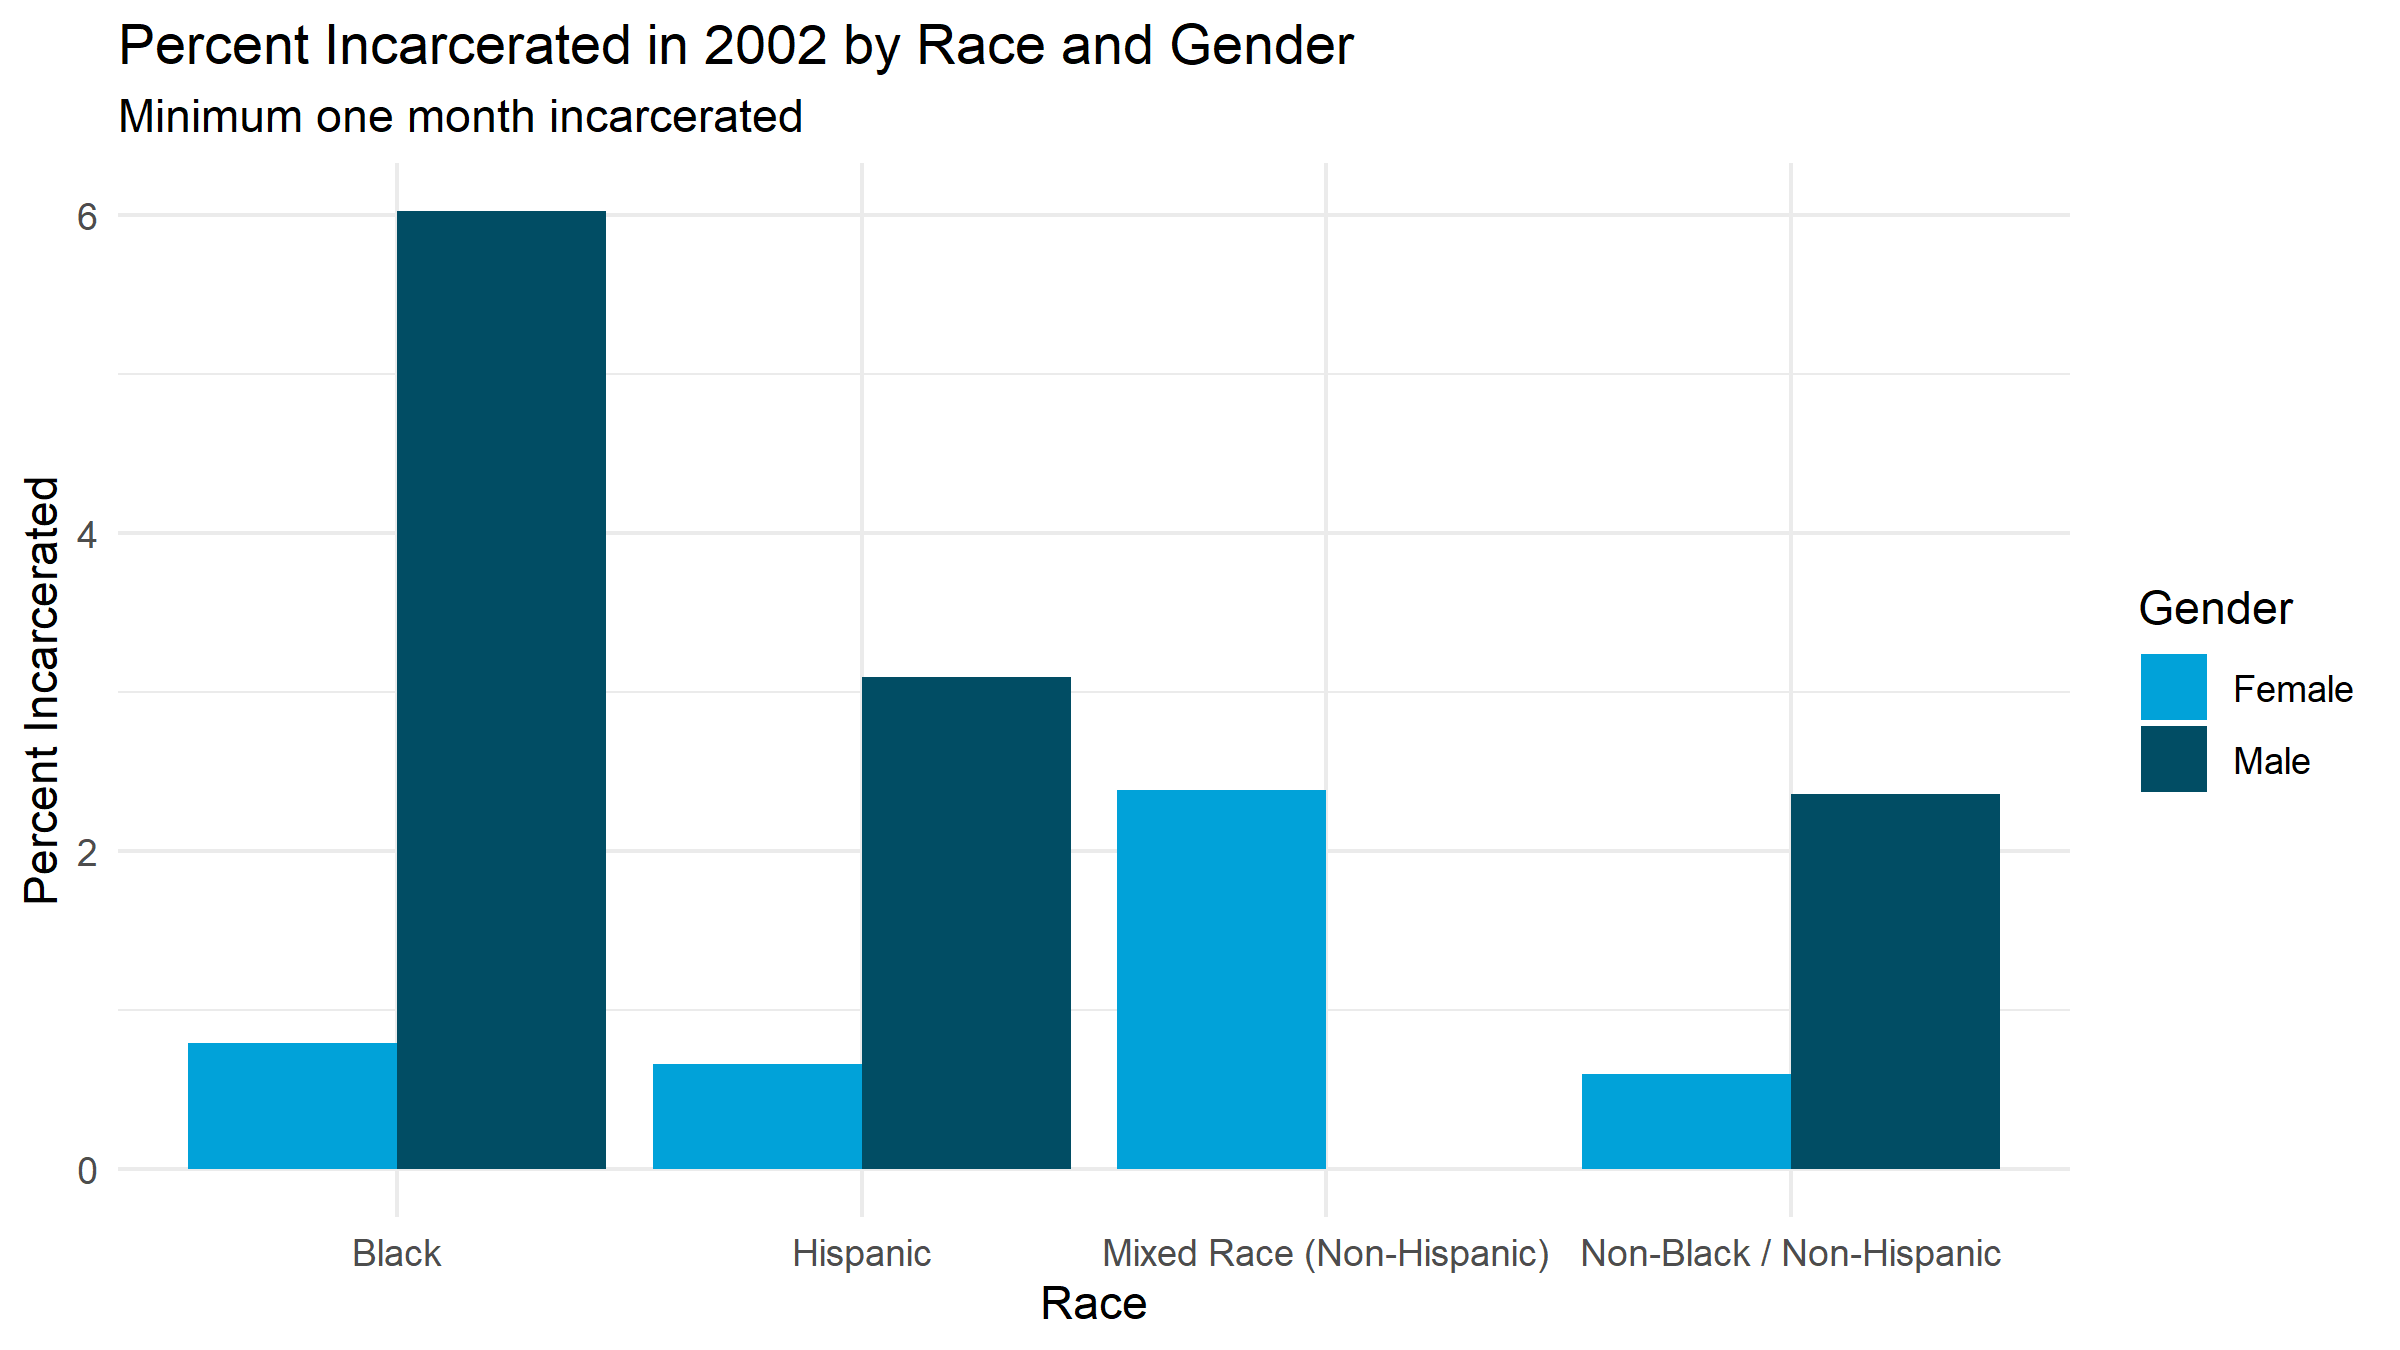
\includegraphics[width=.85\textwidth]{incarcerationpct_by_racegender}
    \end{center}
    \caption{Incarceration Rate in 2002 by Race and Gender}
    \label{fig:graph}
\end{figure}

This information is further presented in Table 1, where incarceration percent is presented by race and gender. As mentioned, with the exception of the mixed race non-Hispanic category, male incarceration percent is generally an order of magnitude larger than for their same demographic females. Black males had a rate of 6.03$\%$ for the year, while Hispanic and non-Black non-Hispanic groups had percents of 3.09$\%$ and 2.36$\%$, respectively. 

\begin{table}[H]

\caption{\label{tab:tab:summarystats}Percent Incarcerated in 2002 by Race and Gender}
\centering
\begin{tabular}[t]{lrrrr}
\toprule
Gender & Black & Hispanic & Mixed Race Non Hispanic & Non Black Non Hispanic\\
\midrule
\cellcolor{gray!6}{Female} & \cellcolor{gray!6}{0.7922535} & \cellcolor{gray!6}{0.6622517} & \cellcolor{gray!6}{2.380952} & \cellcolor{gray!6}{0.5979761}\\
Male & 6.0273973 & 3.0949840 & 0.000000 & 2.3560209\\
\bottomrule
\end{tabular}
\end{table}


Table 2 shows the regression of percent incarcerations on the racial and gender categorical variables. Similar to the results indicated above, males had an average incarceration rate 2.76 percentage points higher than females, and Black individuals had higher associated incarceration rate than Hispanic (1.51 percentage points higher), mixed race non-Hispanic (2.10 more) and non-Black non-Hispanic (1.92 more), holding all else fixed. As we previously saw, the regression indicates the highest associated incarceration of any gender and racial group is Black males. Note that coeffecients are scaled to a percent scale out of 100. 
 

% Table created by stargazer v.5.2.2 by Marek Hlavac, Harvard University. E-mail: hlavac at fas.harvard.edu
% Date and time: Wed, Feb 16, 2022 - 9:48:12 AM
\begin{table}[!htbp] \centering 
  \caption{Regression Output. Omitted category is Black Females.} 
  \label{tab:regression} 
\begin{tabular}{@{\extracolsep{5pt}}lc} 
\\[-1.8ex]\hline 
\hline \\[-1.8ex] 
 & \multicolumn{1}{c}{\textit{Dependent variable:}} \\ 
\cline{2-2} 
\\[-1.8ex] & Incarceration Rate in 2002 \\ 
\hline \\[-1.8ex] 
 Hispanic & $-$1.511$^{***}$ \\ 
  & (0.495) \\ 
  & \\ 
 Mixed Race (Non-Hispanic) & $-$2.101 \\ 
  & (1.323) \\ 
  & \\ 
 Non-Black / Non-Hispanic & $-$1.923$^{***}$ \\ 
  & (0.422) \\ 
  & \\ 
 Male & 2.763$^{***}$ \\ 
  & (0.304) \\ 
  & \\ 
 Constant & 2.005$^{***}$ \\ 
  & (0.332) \\ 
  & \\ 
\hline \\[-1.8ex] 
Observations & 8,621 \\ 
R$^{2}$ & 0.012 \\ 
Adjusted R$^{2}$ & 0.012 \\ 
Residual Std. Error & 14.135 (df = 8616) \\ 
F Statistic & 27.193$^{***}$ (df = 4; 8616) \\ 
\hline 
\hline \\[-1.8ex] 
\textit{Note:}  & \multicolumn{1}{r}{$^{*}$p$<$0.1; $^{**}$p$<$0.05; $^{***}$p$<$0.01} \\ 
\end{tabular} 
\end{table} 


\end{document}
